\section{Calibration}
\label{sec:calib}

\subsection{Principle}

\begin{figure}
\centering
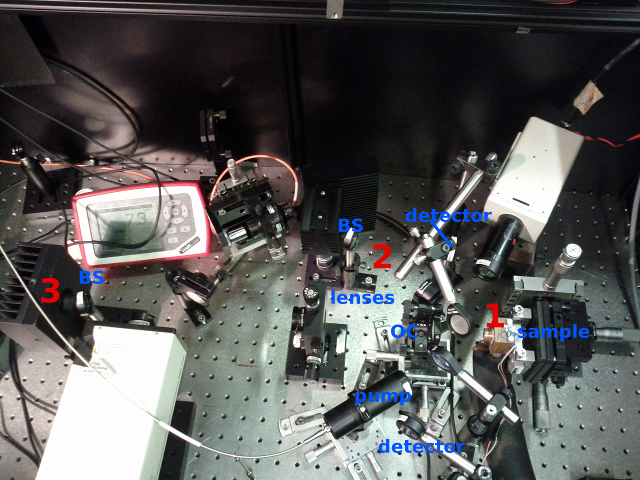
\includegraphics[width=12.5cm]{img/calib_setup.png}
\caption{In order to calibrate the setup we have to
measure the actually present power at the indicated positions 1--3.}
\label{img:calib_setup}
\end{figure}

Figure~\ref{img:calib_setup} shows a photograph of the setup.
Before we can use it to characterize samples,
we have to characterize the setup first.
Following the beam path,
we start with the lens system indicated as \emph{pump}.
This input beam is targeted at the sample.
Part of this pump beam is sampled by a beam sampler (BS),
a glas plate with high damage threshold and
anti reflective coating on one side.
This sampled light is directed towards a detector.
The pump light is reflected off the sample,
collimated by a lens,
and again sampled as for the input.
The lasing output passes the output coupler (OC),
a collimating lens,
and another beam sampler (coated for the emission wavelength).
This beam sampler we eventually use to record the spectrum of the emission.

In order to calibrate this setup we need to know
how to correlate the readings of the single detectors
with the actually present powers.
For this we place the thermal power meter at
the four indicated positions.
With the thermal power meter we can validate
the setup up to $40\,\mathrm{W}$, in principle.

Position 1 requires to remove the sample.
We're interested in the correlation between the readings
of the detector after the beam sampler
and the measurements at the sample position.
From this same measurement we can also extract
a look-up-table what current setting of the pump laser
corresponds to what output power.

On position 2 we measure the beam power present after the collimating lens.
This we relate with the readings of the detector after the beam sampler,
gathered during the measurements at position 3 (below).
Make sure (IR-viewer) you capture
all of the reflected light
within the aperture of the power meter.
Clipping during the calibration
renders everything else useless.

At position 3
we need two measurements:
once with and once without the beam sampler.
The difference between these two measurements
lets us correct for the fraction of light
the beam sampler directs away.

The pump order during calibration is a ramp
(not random sampling
as for the measurement routine,
section~\ref{sec:routine}).
As shown in Fig.~\ref{img:random_sampling_ramp_heatsink}
this way we arrive in a highly repeatable situation,
using the same exact ramp.

\subsection{Implementation}

The routine in \code{exp/meas/routine\_calibration.py}
needs the following 4 files.
The calibration evaluation routine
in \code{exp/eval/calibration.py}
should also clear things up,
what the following comments mean.

Between these measurements
you move only the thermal power meter
to the different positions indicated in Fig.~\ref{img:calib_setup}.
Do not touch the other equipment!
With this procedure
we gauge the photo detectors
(after beam splitters to protect from high power)
to the thermal power meter.
When placing the thermal power meter,
you have to make sure the exposure is below its damage threshold.
A Thorlabs thermal power meter S314C,
for example,
has a power range limited up to 40W.

\paragraph{\code{1\_pump\_calib.csv}}:\\
Place the thermal power meter at the sample position; position 1.
Choose the variable \code{pump\_end} equal to
the pump current corresponding to
the maximally allowed pump power
(or less, to be on the safe side).
(Note: \code{pump\_end} will be a lower value
than during actual operation.
This is made possible
because there is a linear relation
between pump current and the power seen at position 1.
We're going to extrapolate based on this linear relationship.
Ensure yourself, this is actually linear!
(Otherwise you have to find a new solution how to do the job.))

\paragraph{\code{2\_refl\_calib.csv}}:\\
Thermal power meter goes in the reflection channel,
between collimating lens and beam sampler; position 2.
Variable \code{pump\_end} now determines
up to what power you can calibrate the setup over all.
Make sure the power exposure at this point
doesn't exceed the power range of the power meter.
Caveat:
If you replace the sample under test
without changing the alignment,
you can -- in principle -- use an old calibration.
But, if this sample has a higher reflectivity,
you run the risk of entering an uncalibrated range.

\paragraph{\code{3\_emission\_calib.csv}}:\\
Thermal power meter goes
at its final position in the laser emission path --
position 3 --
without the spectrometer beam sampler.

\paragraph{\code{4\_emission\_calib.csv}}:\\
Thermal power meter goes
at its final position in the laser emission path --
position 3 --
with the spectrometer beam sampler in place.
Measurement 3 and 4 allow you to find the influence of said beam sampler.

In practice you will probably gather these four measurement in reverse order.
After you have conducted the measurements
(e.g. with \code{routine\_measurement.py}),
you run this script for 4,
remove the spectrometer beam sampler and measure 3,
and so on.
This way you're sure
to account for the actual alignment
present during the measurements.


\subsection{Evaluation}

The example routine \code{exp/eval/calibration.py}
works with these mentioned files.
It is easiest to look at the code
and learn based on the comments
provided alongside.
The \code{main()} function
in these scripts
you can use
to calibrate one of the specific parts manually.
